\chapter{单态、贝尔不等式与不可克隆}

\lectureoverview{一个相对负号将仅仅相关的双自旋态转变为旋转不变的 singlet。我们通过计算其总自旋来识别该态，利用其完美的反关联来构建贝尔实验，并将经典命题转化为量子投影算符。由此得到的概率违反贝尔的经典计数不等式。关于定域性、实验时序和不确定性的问题随后引向线性量子力学的第二个推论：未知态无法被通用克隆机复制。}

\section{一个符号能带来什么差别？}

考虑两个电子，并在基态中省略张量积符号：
\begin{equation}
  \ket{ud}\equiv\ket{u}_1\otimes\ket{d}_2,
  \qquad
  \ket{du}\equiv\ket{d}_1\otimes\ket{u}_2.
\end{equation}
两个特别简单的叠加态仅相差一个符号，
\begin{equation}
  \ket{\psi_\pm}
  =
  \frac{\ket{ud}\pm\ket{du}}{\sqrt2}.
  \label{eq:l05-two-signs}
\end{equation}
因子 \(1/\sqrt2\) 使总概率为 1。在任一态中，沿第三轴测量都会得到相反的答案：若电子 1 为上，则电子 2 为下，反之亦然。因此，仅凭该关联无法探测到符号。然而，这两个态在物理上是不同的。

计算将反复使用泡利作用
\begin{align}
  \sigma_1\ket{u}&=\ket{d},&
  \sigma_1\ket{d}&=\ket{u},\nonumber\\
  \sigma_2\ket{u}&=i\ket{d},&
  \sigma_2\ket{d}&=-i\ket{u},\nonumber\\
  \sigma_3\ket{u}&=\ket{u},&
  \sigma_3\ket{d}&=-\ket{d}.
  \label{eq:l05-pauli-actions}
\end{align}
我们保留 \(\sigma_i\) 表示作用于电子 1 的算符，并引入作用于电子 2 的相同族 \(\tau_i\)。

\begin{figure}[htbp]
\centering
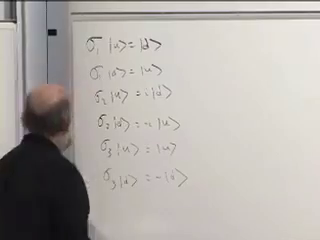
\includegraphics[width=0.62\linewidth]{lecture_05_figure_02.png}
\caption{整个比较中使用的完整泡利作用表。}
\lectureframe{00:03:15}
\end{figure}

在两个态中，任一分自旋都没有优先方向：
\begin{equation}
  \expect{\sigma_i}_{\psi_\pm}=0,
  \qquad
  \expect{\tau_i}_{\psi_\pm}=0,
  \qquad i=1,2,3.
  \label{eq:l05-local-zero}
\end{equation}
例如，对加态所要求的显式检验给出
\begin{align}
  \bra{\psi_+}\sigma_3\ket{\psi_+}
  &=
  \frac12
  \bigl(\bra{ud}+\bra{du}\bigr)
  \bigl(\ket{ud}-\ket{du}\bigr)\nonumber\\
  &=
  \frac12(1-1)=0.
  \label{eq:l05-sigma3-expectation}
\end{align}
交叉项消失，因为 \(\braket{ud}{du}=0\)。

\begin{figure}[htbp]
\centering
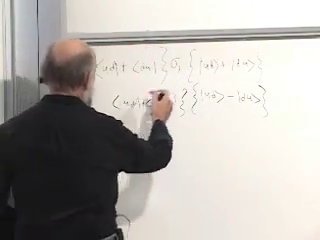
\includegraphics[width=0.78\linewidth]{lecture_05_figure_03.png}
\caption{加态的期望值通过作用 \(\sigma_3\) 并利用正交性来计算。}
\lectureframe{00:07:00}
\end{figure}

\begin{classroomqa}
\lecturetimestamp{00:07:13}
\audiencequestion{期望值为零是否意味着单个自旋可以被测量为零值？}
\lecturerresponse{不。一个自旋的分量只有结果 \(+1\) 和 \(-1\)；\(\sigma_i\) 没有零本征值。方程~\eqref{eq:l05-local-zero} 说明重复测量如同公平的掷硬币，而不是说任何单次结果为零。}
\end{classroomqa}

因此，第一个看似合理的诊断失败了。局域平均值无法看到相对符号，所以我们必须测量这对粒子的某个性质。

\section{总自旋选出单态}

这对粒子的磁矩由矢量和表示
\begin{equation}
  \boldsymbol{\Sigma}
  =
  \boldsymbol{\sigma}+\boldsymbol{\tau}.
\end{equation}
其第三分量湮灭两个基矢：
\begin{align}
  (\sigma_3+\tau_3)\ket{ud}
  &=(1-1)\ket{ud}=0,\nonumber\\
  (\sigma_3+\tau_3)\ket{du}
  &=(-1+1)\ket{du}=0.
\end{align}
因此，
\begin{equation}
  (\sigma_3+\tau_3)\ket{\psi_\pm}=0.
\end{equation}
两种符号选择在每次试验中总第三分量均为零。

第一分量将它们区分开来。由方程~\eqref{eq:l05-pauli-actions}，
\begin{align}
  (\sigma_1+\tau_1)\ket{ud}
  &=\ket{dd}+\ket{uu},\nonumber\\
  (\sigma_1+\tau_1)\ket{du}
  &=\ket{uu}+\ket{dd}.
\end{align}
因此
\begin{align}
  (\sigma_1+\tau_1)\ket{\psi_+}
  &=
  \sqrt2\bigl(\ket{uu}+\ket{dd}\bigr),\nonumber\\
  (\sigma_1+\tau_1)\ket{\psi_-}
  &=0.
  \label{eq:l05-total-x}
\end{align}
加态对该可观测量可能具有零期望值，但它并不是其零本征值本征态。

\begin{classroomqa}
\lecturetimestamp{00:13:02}
\audiencequestion{当态未被湮灭时，总分量可以有哪些结果？}
\lecturerresponse{每个分量的答案为 \(+1\) 或 \(-1\)，因此它们的和可以是 \(2\)、\(0\) 或 \(-2\)。零期望并不强制每次运行都为零。}
\end{classroomqa}

第二分量完成了检验。其 \(i\) 因子在反对称组合中相消：
\begin{equation}
  (\sigma_2+\tau_2)\ket{\psi_-}=0.
\end{equation}
因此所有三个分量都湮灭减态，
\begin{equation}
  \bigl(\boldsymbol{\sigma}+\boldsymbol{\tau}\bigr)
  \cdot\hat n\,\ket{\psi_-}=0
  \qquad\text{for every unit vector }\hat n.
  \label{eq:l05-singlet-any-axis}
\end{equation}

\begin{figure}[htbp]
\centering
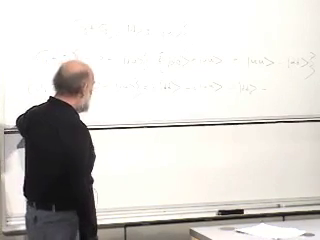
\includegraphics[width=0.84\linewidth]{lecture_05_figure_06.png}
\caption{逐分量相消将减态识别为总自旋为零。}
\lectureframe{00:16:30}
\end{figure}

反对称态 \(\ket{\psi_-}\) 是 \emph{singlet}。它具有旋转不变性：每个轴都给出相同的总自旋答案，零。方程~\eqref{eq:l05-two-signs} 中的对称态属于三重态部分。

\begin{classroomqa}
\lecturetimestamp{00:19:06}
\audiencequestion{相反自旋的结果仅平均成立吗？}
\lecturerresponse{对于单态，它在每次试验中都成立。方程~\eqref{eq:l05-singlet-any-axis} 是本征矢方程，因此对两个粒子测量同一分量总是给出和为本征值零的答案。}
\end{classroomqa}

\begin{classroomqa}
\lecturetimestamp{00:19:36}
\audiencequestion{为什么另一个态被称为三重态？}
\lecturerresponse{该名称来自总自旋为一的多重态中的三个态。其推导被推迟；当前计算只需要对称态与一维单态部分之间的对比。}
\end{classroomqa}

如果Bob测量他电子自旋的任意一个分量，他立刻就知道Alice测量她自己电子的同一分量会得到什么结果：她的答案必定相反。这就是一个Einstein--Podolsky--Rosen关联。一对隐藏的硬币也可以携带相反的结果，但只对预先安排好的一个问题成立。单态对无论选择哪条空间轴都提供完美的反关联。

\begin{classroomqa}
\lecturetimestamp{00:20:55}
\audiencequestion{Einstein、Podolsky和Rosen最先发现了纠缠吗？}
\lecturerresponse{不是。Schrödinger讨论过这一现象并引入了纠缠这一术语。EPR论证使远距离关联问题变得格外尖锐。}
\end{classroomqa}

\begin{classroomqa}
\lecturetimestamp{00:23:50}
\audiencequestion{这种瞬时关联违反因果律吗？由哪位观察者先测量有关系吗？}
\lecturerresponse{没有可用的信息被传递。无论Bob是否测量，在每个惯性参考系的先后次序中，Alice的本地结果都保持各半。她只有在通过普通经典信道收到Bob的结果之后才能验证这种关联，而经典信道无法超过光速。}
\end{classroomqa}

\section{Bell不等式是经典计数}

Bell结果的地位可能让人觉得不稳定。有些时候它显得是量子力学最深刻的特征；另一些时候它又显得只是形式体系的一个不可避免的推论。Bell本人以及Feynman都能表达这两种态度。然而，这个不等式是初等的。令人惊讶之处在于它被违反。

取一组普通的对象。每个对象可能具有或不具有三个性质\(A\)、\(B\)和\(C\)。令\(N(A,\neg B)\)表示具有\(A\)但不具有\(B\)的对象的数目。经典集合逻辑蕴含
\begin{equation}
  N(A,\neg B)+N(B,\neg C)
  \geq
  N(A,\neg C).
  \label{eq:l05-bell-count}
\end{equation}
证明就是集合包含关系
\begin{equation}
  A\cap C^{c}
  \subseteq
  (A\cap B^{c})\cup(B\cap C^{c}).
  \label{eq:l05-set-inclusion}
\end{equation}
确实，\(A\cap C^c\)的一个元素要么属于\(B\)，要么不属于。在第一种情形下它属于\(B\cap C^c\)；在第二种情形下它属于\(A\cap B^c\)。对并集计数只可能多算左边集合中的元素。

\begin{figure}[htbp]
\centering
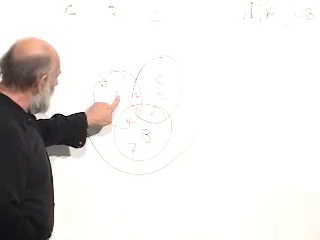
\includegraphics[width=0.78\linewidth]{lecture_05_figure_07.png}
\caption{黑板上的证明把三个相互重叠的经典子集划分为非负的区域。}
\lectureframe{00:31:15}
\end{figure}

等价地，用非负整数\(N_i\)标记三集合图中互不重叠的区域。方程~\eqref{eq:l05-bell-count}的两边都包含\(A\cap C^c\)所要求的区域，而左边还包含额外的非负区域。这里没有引入任何量子内容。这是关于子集和普通逻辑备择项的定理。

\section{把集合陈述转化为自旋实验}

制备许多处于单态的独立电子对，并定义关于电子1的三个命题：
\begin{align}
  A&:\ \text{spin 1 is up at }0^\circ\text{, along the third axis},\nonumber\\
  B&:\ \text{spin 1 is up at }45^\circ\text{ in the }zx\text{-plane},\nonumber\\
  C&:\ \text{spin 1 is up at }90^\circ\text{, along the first axis}.
  \label{eq:l05-abc}
\end{align}

\begin{figure}[htbp]
\centering
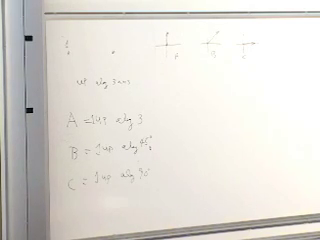
\includegraphics[width=0.82\linewidth]{lecture_05_figure_08.png}
\caption{这三个自旋命题固定在同一平面内的\(0^\circ\)、\(45^\circ\)和\(90^\circ\)处。}
\lectureframe{00:39:00}
\end{figure}

在单态中，关于电子1的命题的否定可以改写为关于电子2的肯定命题。例如，
\begin{align}
  \neg B
  &:\ \text{spin 1 is down at }45^\circ\nonumber\\
  &\Longleftrightarrow
  \text{spin 2 is up at }45^\circ.
\end{align}
同样，\(\neg C\)变成电子2在\(90^\circ\)处为自旋向上的陈述。

\begin{classroomqa}
\lecturetimestamp{00:40:04}
\audiencequestion{\(\neg C\)是否使电子2在\(90^\circ\)处为自旋向下？}
\lecturerresponse{不是。首先否定\(C\)：电子1在\(90^\circ\)处为自旋向下。完美的单态反关联随后使电子2沿同一轴为自旋向上。这两次反转必须分开处理。}
\end{classroomqa}

对于大系综，计数与概率只相差所制备电子对的共同数目。旋转不变性还给出
\begin{equation}
  P(A,\neg B)=P(B,\neg C),
\end{equation}
因为第二个实验是第一个实验旋转\(45^\circ\)的结果。因此Bell的经典不等式将要求
\begin{equation}
  2P(A,\neg B)\geq P(A,\neg C).
  \label{eq:l05-bell-probability}
\end{equation}
我们现在需要一种高效的方法来计算这些概率。

\section{命题变成投影算符}

在普通的三维向量空间中，投影算符会移除垂直于所选子空间的每一个分量。一维投影算符把向量正交投影到一条直线上；二维投影算符把它投影到一个平面上。如果\(P\)投影到指定的子空间，则
\begin{equation}
  P\ket{\alpha}=\ket{\alpha_P}.
\end{equation}

\begin{figure}[htbp]
\centering
\includegraphics[width=0.76\linewidth]{lecture_05_figure_04.png}
\caption{几何投影及其算符记号被并排展开。}
\lectureframe{00:49:53}
\end{figure}

\begin{figure}[htbp]
\centering
\begin{tikzpicture}[scale=1.05,>=Latex]
  \draw[->] (-0.25,0)--(4.0,0);
  \draw[thick] (-0.25,-0.25)--(3.55,2.6);
  \draw[->,very thick] (0,0)--(2.25,3.05)
    node[above] {\(\ket{\alpha}\)};
  \coordinate (P) at (2.72,1.98);
  \draw[dashed] (2.25,3.05)--(P);
  \draw[->,very thick] (0,0)--(P)
    node[right] {\(\ket{\alpha_P}\)};
  \node[below right] at (3.1,2.25) {projected subspace};
\end{tikzpicture}
\caption{对投影几何的清晰重构。}
\end{figure}

在单自旋Hilbert空间中，命题\(\sigma_3=+1\)对应于由\(\ket{u}\)张成的一维子空间。其投影算符的作用为
\begin{equation}
  P_{\sigma_3=+1}
  \begin{pmatrix}\alpha\\\beta\end{pmatrix}
  =
  \begin{pmatrix}\alpha\\0\end{pmatrix},
  \qquad
  P_{\sigma_3=-1}
  \begin{pmatrix}\alpha\\\beta\end{pmatrix}
  =
  \begin{pmatrix}0\\\beta\end{pmatrix}.
  \label{eq:l05-projector-actions}
\end{equation}

\begin{classroomqa}
\lecturetimestamp{00:49:55}
\audiencequestion{第一个投影算符是否报告矢量在竖直轴上能达到多高？}
\lecturerresponse{不。它只是丢弃正交的系数\(\beta\)。这些分量是希尔伯特空间中的振幅，而不是自旋的普通空间坐标。}
\end{classroomqa}

\begin{figure}[htbp]
\centering
\includegraphics[width=0.78\linewidth]{lecture_05_figure_05.png}
\caption{投影算符先作用于一般的旋量，然后写成显式的矩阵。}
\lectureframe{00:51:40}
\end{figure}

矩阵形式为
\begin{equation}
  P_{\sigma_3=+1}
  =
  \begin{pmatrix}1&0\\0&0\end{pmatrix}
  =
  \frac{I+\sigma_3}{2}.
  \label{eq:l05-p3}
\end{equation}
同样的构造沿任意单位矢量\(\hat n\)都成立：
\begin{equation}
  P_{\boldsymbol{\sigma}\cdot\hat n=+1}
  =
  \frac{I+\boldsymbol{\sigma}\cdot\hat n}{2}.
  \label{eq:l05-pn}
\end{equation}

\begin{classroomqa}
\lecturetimestamp{00:53:09}
\audiencequestion{投影到\(\sigma_1=+1\)上的投影算符是什么？}
\lecturerresponse{在方程~\eqref{eq:l05-p3}中用\(\sigma_1\)替换\(\sigma_3\)：\(P_{\sigma_1=+1}=(I+\sigma_1)/2\)。}
\end{classroomqa}

玻恩规则现在有了一个有用的命题形式：
\begin{equation}
  P(\mathcal A\text{ is true in }\ket{\psi})
  =
  \bra{\psi}P_{\mathcal A}\ket{\psi}.
  \label{eq:l05-projector-born}
\end{equation}
对于归一化的旋量\(\ket{\psi}=(\alpha,\beta)^T\)，方程~\eqref{eq:l05-projector-born}在\(P_{\sigma_3=+1}\)下给出\(|\alpha|^2\)，完全符合预期。

这种语言揭示了经典命题与量子命题之间的区别。在经典逻辑中，一个性质对应于一个集合的子集。在量子力学中，一个性质对应于希尔伯特空间的一个子空间，或者等价地对应于它的投影算符。子集与矢量子空间并不遵循相同的格运算；贝尔的矛盾正是从这一区别中产生的。

\subsection{联合贝尔投影算符}

对于\(A\wedge\neg B\)，电子1必须沿第三轴向上，而电子2必须沿
\begin{equation}
  \hat n_{45}=\frac{\hat x+\hat z}{\sqrt2}.
\end{equation}向上。
第二个自旋的相关分量为
\begin{equation}
  \boldsymbol{\tau}\cdot\hat n_{45}
  =
  \frac{\tau_1+\tau_3}{\sqrt2}.
\end{equation}
因此联合投影算符为
\begin{equation}
  P_{A\wedge\neg B}
  =
  \frac{I+\sigma_3}{2}
  \frac{I+(\tau_1+\tau_3)/\sqrt2}{2}.
  \label{eq:l05-joint-projector}
\end{equation}

\begin{classroomqa}
\lecturetimestamp{00:59:18}
\audiencequestion{为什么\(45^\circ\)自旋分量中有一个因子\(1/\sqrt2\)？}
\lecturerresponse{该方向必须是单位矢量。它的第一轴和第三轴分量都是\(1/\sqrt2\)，所以相应的可观测量是\((\tau_1+\tau_3)/\sqrt2\)。}
\end{classroomqa}

\begin{classroomqa}
\lecturetimestamp{01:00:52}
\audiencequestion{整个表达式\(I+\boldsymbol{\tau}\cdot\hat n_{45}\)是否除以二？}
\lecturerresponse{是的。投影算符是\(\bigl(I+\boldsymbol{\tau}\cdot\hat n_{45}\bigr)/2\)；因子\(1/2\)乘的是整个分子。}
\end{classroomqa}

方程~\eqref{eq:l05-joint-projector}中的两个因子作用于不同的张量因子，因此对易。先施加两者，会先移除电子1向下的所有分量，然后移除电子2沿\(\hat n_{45}\)向下的所有剩余分量。

\section{量子数反转不等式}

令
\begin{equation}
  \ket{\psi_s}
  =
  \frac{\ket{ud}-\ket{du}}{\sqrt2}
\end{equation}
表示单态。从
\begin{equation}
  P(A,\neg B)
  =
  \bra{\psi_s}P_{A\wedge\neg B}\ket{\psi_s}.
\end{equation}
开始。因子\((I+\sigma_3)/2\)消灭\(\ket{du}\)并留下\(\ket{ud}/\sqrt2\)。第二个因子随后给出
\begin{align}
  \frac{I+(\tau_1+\tau_3)/\sqrt2}{2}\ket{ud}
  &\notag\\[-0.3em]
  &=
  \frac12
  \left[
    \ket{ud}
    +\frac{\ket{uu}-\ket{ud}}{\sqrt2}
  \right]\nonumber\\
  &=
  \frac12
  \Biggl[
    \left(1-\frac1{\sqrt2}\right)\ket{ud}
  \nonumber\\
  &\qquad
    +\frac1{\sqrt2}\ket{uu}\Biggr].
  \label{eq:l05-projector-action}
\end{align}
\(\ket{uu}\)项与单态左矢的 overlap 为零，而剩余的归一化因子给出
\begin{equation}
  P(A,\neg B)
  =
  \frac14\left(1-\frac1{\sqrt2}\right).
  \label{eq:l05-pab}
\end{equation}

\begin{figure}[htbp]
\centering
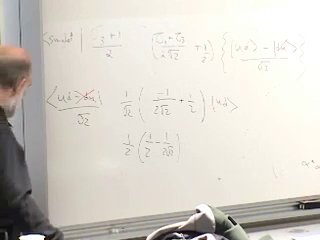
\includegraphics[width=0.88\linewidth]{lecture_05_figure_09.png}
\caption{投影算符计算保留了\(\ket{ud}\)的 overlap，并丢弃了正交的\(\ket{uu}\)贡献。}
\lectureframe{01:08:20}
\end{figure}

旋转不变性给出下一对方向的相同结果：
\begin{equation}
  P(B,\neg C)
  =
  \frac14\left(1-\frac1{\sqrt2}\right).
\end{equation}
对于\(A\wedge\neg C\)，第二轴就是第一空间轴，所以
\begin{equation}
  P_{A\wedge\neg C}
  =
  \frac{I+\sigma_3}{2}\frac{I+\tau_1}{2}.
\end{equation}
第一个因子再次留下\(\ket{ud}/\sqrt2\)。\(\tau_1\)项产生\(\ket{uu}\)，它与单态左矢正交，而恒等项存活下来。因此
\begin{equation}
  P(A,\neg C)=\frac14.
  \label{eq:l05-pac}
\end{equation}
综合这三个结果，
\begin{equation}
  \underbrace{
  P(A,\neg B)+P(B,\neg C)
  }_{\frac12(1-1/\sqrt2)\approx0.146}
  <
  \underbrace{
  P(A,\neg C)
  }_{\frac14=0.25}.
  \label{eq:l05-bell-violation}
\end{equation}

\begin{figure}[htbp]
\centering
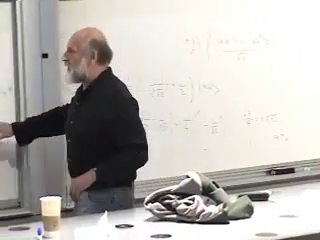
\includegraphics[width=0.84\linewidth]{lecture_05_figure_10.png}
\caption{完成的板书计算显示出较小的贝尔不等式左侧和较大的右侧。}
\lectureframe{01:12:15}
\end{figure}

方程~\eqref{eq:l05-bell-violation}反转了方程~\eqref{eq:l05-bell-probability}。结论并不是量子力学自相矛盾。而是单态关联不可能来自一个局域经典模型，在该模型中，三个自旋命题都具有普通的集合论真值，且独立于远处的测量选择。经典模拟若要再现这些关联，只能放弃至少一条贝尔假设，其中最显著的是局域性。

\section{贝尔实验检验的是什么}

量子力学已经预言了这种违反。实验还必须堵住经典逃逸路径，即一个探测器告知另一个探测器它遇到了什么设置或结果。两翼应当相距足够远，且选择和探测在时间上足够接近，使得光速信号无法在它们之间传播。阿斯佩的实验在操作上令人信服地实现了这种时间安排和隔离。

\begin{classroomqa}
\lecturetimestamp{01:13:15}
\audiencequestion{如果量子力学已经给出了答案，贝尔实验还教给了我们什么吗？}
\lecturerresponse{它们检验了自然界是否在这个精确的关联实验中遵循量子预言，并且关键的是，使两个测量翼在相关的光传播时间上相互独立。实验控制和计时本身就是重大的成就。}
\end{classroomqa}

\begin{classroomqa}
\lecturetimestamp{01:18:19}
\audiencequestion{在爱因斯坦讨论幽灵般的超距作用之后，贝尔补充了什么？}
\lecturerresponse{贝尔给出了一个定量不等式。他确定了一个可行的关联实验，其量子预言排除了局域经典底层描述，而不是把异议停留在哲学不安的层面。贝尔对于这是不可避免还是意义深远始终态度矛盾，并且越来越愿意质疑标准量子力学。}
\end{classroomqa}

粒子可能相距数英里，却仍共享一个联合态，但这仍然是对小系统的量子实验。环境相互作用往往会破坏所需的相位关系。空气分子、杂散光子和热扰动会与这对粒子发生纠缠，因此分离必须在寒冷且隔离良好的环境中进行。

\begin{classroomqa}
\lecturetimestamp{01:19:53}
\audiencequestion{一个共同态延展到很大距离，是否就使这成为一个宏观量子客体？}
\lecturerresponse{更恰当的描述是相距很远的小量子系统。它们的间距可以很大，但保持其联合波函数会变得越来越精细，因为与环境不受控制的相互作用会破坏有用的相干性。两个普通保龄球并不能提供同样的实验。}
\end{classroomqa}

\begin{classroomqa}
\lecturetimestamp{01:21:23}
\audiencequestion{测量一个粒子能否揭示关于另一个粒子的互补信息，从而规避不确定性原理？}
\lecturerresponse{例如，可以测量一个粒子的位置和另一个粒子的动量。这并不是对同一个粒子同时测量非对易可观测量。对单个系统的不确定性限制并未被规避。}
\end{classroomqa}

\section{乘积何时表示“与”？}

贝尔计算将两个投影算符相乘。只有当命题相容时，这才表示合取。

\begin{classroomqa}
\lecturetimestamp{01:22:39}
\audiencequestion{为什么两个投影算符的乘积表示逻辑词“与”？}
\lecturerresponse{因为这两个投影算符对易。一个作用于电子1，另一个作用于电子2，所以它们的顺序无关紧要，两个性质可以一起检验。对于单个电子，\((I+\sigma_3)/2\)和\((I+\sigma_1)/2\)不对易；沿两个轴都自旋向上并不是这种意义上的联合确定命题。}
\end{classroomqa}

这是量子命题偏离普通子集的又一处。经典交集总是存在。由乘积投影算符表示的量子类似物，只有在相关子空间相容时才具有预期的逻辑含义。

同一讨论也指向测量本身。测量装置具有指针态。如果一个向上电子使指针朝一个方向偏转，一个向下电子使它朝另一个方向偏转，那么处于叠加态的电子就与两个指针位置发生纠缠。因此，测量可以作为系统与仪器之间的纠缠来研究。这个问题被推迟，转而讨论一个只使用线性性的更短定理。

\begin{classroomqa}
\lecturetimestamp{01:25:09}
\audiencequestion{把波函数坍缩视为一次测量约束联合态，是否有用？}
\lecturerresponse{这个问题属于测量过程。仪器与被测系统发生纠缠：一个自旋值与一个指针位置相关联，另一个值与另一个指针位置相关联。关于测量的详细讨论被推迟。}
\end{classroomqa}

\section{线性性禁止通用复印机}

关于时间演化只需要一个事实。如果一个物理过程把
\begin{equation}
  \ket{a}\longrightarrow\ket{a'},
  \qquad
  \ket{b}\longrightarrow\ket{b'},
\end{equation}
那么线性性要求
\begin{equation}
  \alpha\ket{a}+\beta\ket{b}
  \longrightarrow
  \alpha\ket{a'}+\beta\ket{b'}.
  \label{eq:l05-linearity}
\end{equation}

普通复印机可以以可控的小误差复制经典信息。量子要求更强：一台固定装置必须复制呈现给它的任意态的全部振幅。这就是为什么不可克隆也被称为不可量子复印原理。

设想一台机器有一个输入端口和两个输出端口。如果它克隆第三轴基，它必须执行
\begin{equation}
  \ket{u}\longrightarrow\ket{uu},
  \qquad
  \ket{d}\longrightarrow\ket{dd}.
  \label{eq:l05-clone-basis}
\end{equation}
这台机器可以向其输出提供能量、质量或电荷；守恒记账并不是障碍。矛盾涉及变换对状态的依赖性。

\begin{figure}[H]
\centering
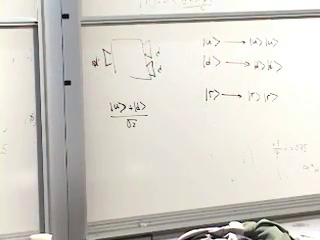
\includegraphics[width=0.86\linewidth]{lecture_05_figure_11.png}
\caption{一个假想的一输入、两输出机器被要求复制两个基态。}
\lectureframe{01:33:45}
\end{figure}

现在输入一个指向右的自旋，
\begin{equation}
  \ket{r}
  =
  \frac{\ket{u}+\ket{d}}{\sqrt2}.
  \label{eq:l05-right-state}
\end{equation}
方程~\eqref{eq:l05-linearity}和\eqref{eq:l05-clone-basis}迫使输出为
\begin{equation}
  \ket{r}
  \longrightarrow
  \frac{\ket{uu}+\ket{dd}}{\sqrt2}.
  \label{eq:l05-linear-output}
\end{equation}
而精确克隆要求两个独立副本：
\begin{align}
  \ket{rr}
  &=
  \ket{r}\otimes\ket{r}\nonumber\\
  &=
  \frac12
  \left(
    \ket{uu}+\ket{ud}+\ket{du}+\ket{dd}
  \right).
  \label{eq:l05-cloned-output}
\end{align}
方程~\eqref{eq:l05-cloned-output}中的混合项在方程~\eqref{eq:l05-linear-output}中不存在。两个输出不同。

\begin{figure}[H]
\centering
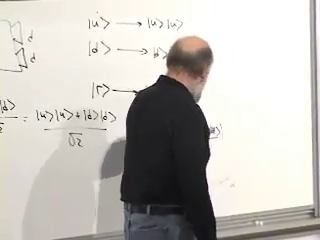
\includegraphics[width=0.72\linewidth]{lecture_05_figure_12.png}
\caption{线性只产生平行自旋项，而两个真正的右指向副本还包含两个混合项。}
\lectureframe{01:35:20}
\end{figure}

\begin{theorem}[No-cloning]
没有任何单一物理机器能够精确克隆每一个未知量子态。
\end{theorem}

\begin{proof}
假设有一台机器按照式~\eqref{eq:l05-clone-basis}克隆正交基态。线性随即将其在二者叠加态上的输出确定为式~\eqref{eq:l05-linear-output}。对同一输入进行精确克隆要求式~\eqref{eq:l05-cloned-output}。由于这两个态矢量不同，所假设的通用机器不可能存在。
\end{proof}

原因在于结构。将\(\ket{\psi}\)送到\(\ket{\psi}\otimes\ket{\psi}\)在振幅中是二次的，而完整量子态的每一种允许演化都是线性的。

\begin{classroomqa}
\lecturetimestamp{01:35:49}
\audiencequestion{该证明是否假设两个输出相互独立？}
\lecturerresponse{是的，因为两个克隆必须是可独立使用的副本。独立系统通过张量积组合，这就是为什么两个右指向副本是\(\ket{r}\otimes\ket{r}\)。不能分别使用的关联输出不是两个克隆。}
\end{classroomqa}

\begin{classroomqa}
\lecturetimestamp{01:37:20}
\audiencequestion{激光似乎通过受激辐射复制光子的态。该论证在哪里失效？}
\lecturerresponse{原子和电磁模式也参与其中。它们的态对输出有贡献，并从通用克隆的角度表现为噪声。近似克隆是可能的，但完美的态无关克隆是不可能的。}
\end{classroomqa}

\begin{classroomqa}
\lecturetimestamp{01:40:24}
\audiencequestion{即使量子信息不能被复制，它能否被转移？}
\lecturerresponse{能。转移是一种不同的操作：原初载体不必保留该态。不可克隆禁止的是最终得到两个独立的完美副本，而不是将态从一个载体移动到另一个载体。}
\end{classroomqa}

\begin{classroomqa}
\lecturetimestamp{01:41:03}
\audiencequestion{输入态必须是未知的吗？}
\lecturerresponse{如果一个态事先已知，人们可以在该态中制备更多系统，或构建一个适配所选正交基的装置。不可能的是用一台机器接受任意输入，并在事先不知道到达的是哪个态的情况下复制它。}
\end{classroomqa}

\begin{classroomqa}
\lecturetimestamp{01:42:35}
\audiencequestion{两个右态表达式中哪一个是机器的实际输出？}
\lecturerresponse{线性强制给出式~\eqref{eq:l05-linear-output}；克隆要求式~\eqref{eq:l05-cloned-output}。它们的不一致正是矛盾所在。}
\end{classroomqa}

\begin{classroomqa}
\lecturetimestamp{01:43:40}
\audiencequestion{纠缠双粒子态所携带的额外信息能否被量化？}
\lecturerresponse{一个自旋的纯态有两个实物理参数。两个分别制备的自旋提供四个，而四维双自旋希尔伯特空间中的一般纯态在去掉归一化和整体相位后则有六个。这些额外态包括纠缠态，其纠缠程度可以用纠缠熵来量化。}
\end{classroomqa}

\enlargethispage{4\baselineskip}
式~\eqref{eq:l05-two-signs}中的符号如今完成了三项任务。它选出了唯一的自旋总量为零的态，提供了违反经典集合不等式的关联，并揭示了线性量子演化与制作两个副本的非线性行为之间的差异。每一项结果都来自将联合态视为其完整张量积空间中的矢量，而不是视为一组预先存在的局域性质的列表。
